\section{Rice Dataset}
Maxwell's implementations were used for the entirety of this dataset.

For the rice dataset, we chose to use the multilayer perceptron (MLP), k-nearest neighbors (KNN), and
random forest (RF) architectures to predict on our dataset.
We chose this because decision trees are a subset of random forests and naive bayes is hard to adapt
to numerical data.

First, we swept over the secondary hyperparameters in each algorithm.
For MLP, we used a training rate of 0.1, a regularization cost of 0.01, and used unbatched gradient
descent.
As shown in Table \ref{tab:rice_nn}, you can see that a model shape of [64, 128, 1] achieved the
highest accuracy.
For RF, we used the set size as a stopping criteria: nodes below the splitting threshold cannot be
split.
As shown in Table \ref{tab:rice_random_forest}, a splitting threshold of 30 achieves the highest
accuracy.

\begin{table}
    \centering
    \begin{tabular}{c|c|c}
        Model Shape    & Epoch & Mean Accuracy \\
        \hline
        [7, 8, 8, 1]   & 765   & 0.930971 \\ \relax
        [7, 2, 1]      & 979   & 0.929921 \\ \relax
        [7, 2, 4, 1]   & 996   & 0.929659 \\ \relax
        [7, 1]         & 670   & 0.929396 \\ \relax
        [7, 16, 16, 1] & 553   & 0.928871 \\ \relax
        [7, 4, 16, 1]  & 735   & 0.928871 \\ \relax
        [7, 2, 16, 1]  & 656   & 0.928871 \\ \relax
        [7, 16, 1]     & 584   & 0.928871 \\ \relax
        [7, 16, 8, 1]  & 757   & 0.928084 \\ \relax
        [7, 8, 2, 1]   & 969   & 0.928084 \\ \relax
        [7, 8, 1]      & 535   & 0.928084 \\ \relax
        [7, 8, 4, 1]   & 638   & 0.928084 \\ \relax
        [7, 16, 2, 1]  & 760   & 0.927822 \\ \relax
        [7, 2, 8, 1]   & 960   & 0.927822 \\ \relax
        [7, 8, 16, 1]  & 748   & 0.927822 \\ \relax
        [7, 16, 4, 1]  & 732   & 0.927822 \\ \relax
        [7, 4, 8, 1]   & 835   & 0.927559 \\ \relax
        [7, 4, 4, 1]   & 993   & 0.927297 \\ \relax
        [7, 4, 1]      & 781   & 0.927034 \\ \relax
        [7, 4, 2, 1]   & 770   & 0.925722 \\ \relax
        [7, 2, 2, 1]   & 999   & 0.887139
    \end{tabular}
    \caption{The results for the hyperparameter tuning step on the MLP architecture trained on the rice
             dataset.
             The best epoch is used for each hyperparameter setting.}
    \label{tab:rice_nn}
\end{table}

                                 
\begin{table}
    \centering
    \begin{tabular}{c|c|c}
        Minimum Splittable Size & ntree & Mean Accuracy \\
        \hline
        30                      & 100   & 0.928215 \\ \relax
        20                      & 100   & 0.927979 \\ \relax
        40                      & 100   & 0.927428 \\ \relax
        50                      & 100   & 0.927008 \\ \relax
        10                      & 50    & 0.926772 \\ \relax
        2                       & 50    & 0.926772 \\ \relax
        5                       & 50    & 0.926772
    \end{tabular}
    \caption{The results for the hyperparameter tuning step on the Random Forest architecture
             trained on the rice dataset.
             The best ntree value is used for each hyperparameter setting.}
    \label{tab:rice_random_forest}
\end{table}

As shown in Figure \ref{fig:rice_knn}, a k value of around 3 or 4 is the best.
This indicates that the dataset doesn't have very strongly mixed classes.
As shown in Figure \ref{fig:rice_nn}, all metrics plateau around 100 epochs in.
As shown in Figure \ref{fig:rice_random_forest}, the metrics rise steeply and then plateau.
The exact values for these penomena can be found in the referenced graphs and in the code.
The best performing model overall was the MLP with an accuracy of 0.93.
This is really close the best performance of random forests, which was 0.928, but this was
significantly higher than the best performace of the KNN architecture, which was 0.89.
This might indicate that the dataset has differently behaved regions, where some areas have more
outliers than others, making KNN models dificult to fit to the dataset.

\begin{figure}
    \centering
    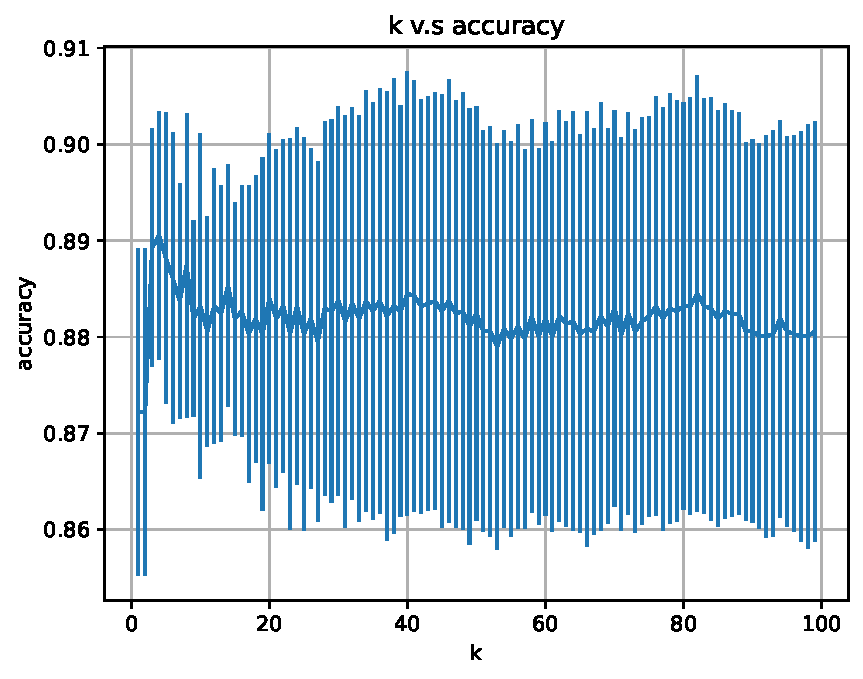
\includegraphics[width=0.30\textwidth]{figures/rice_knn_accuracy.pdf}
    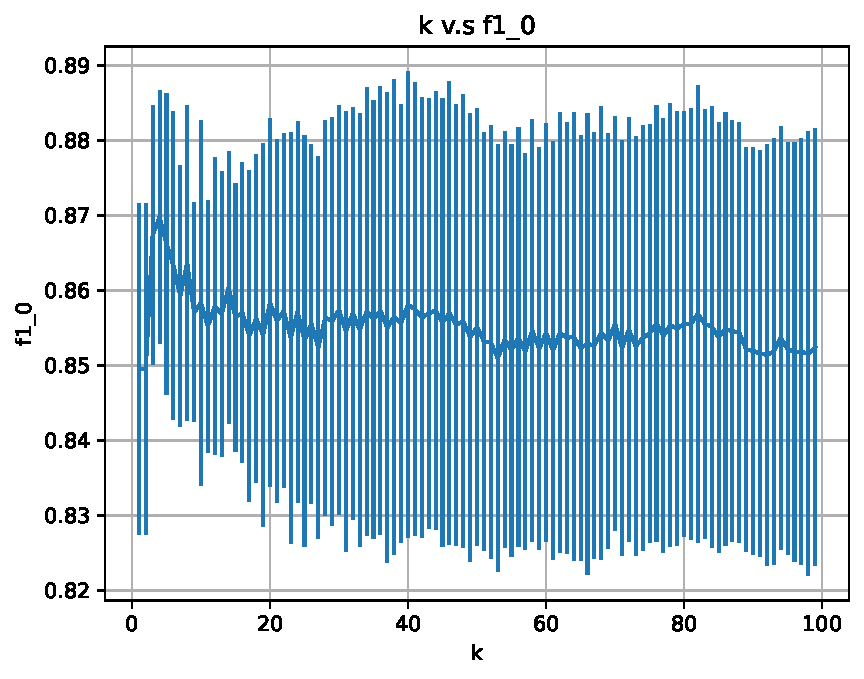
\includegraphics[width=0.30\textwidth]{figures/rice_knn_f1_0.pdf}
    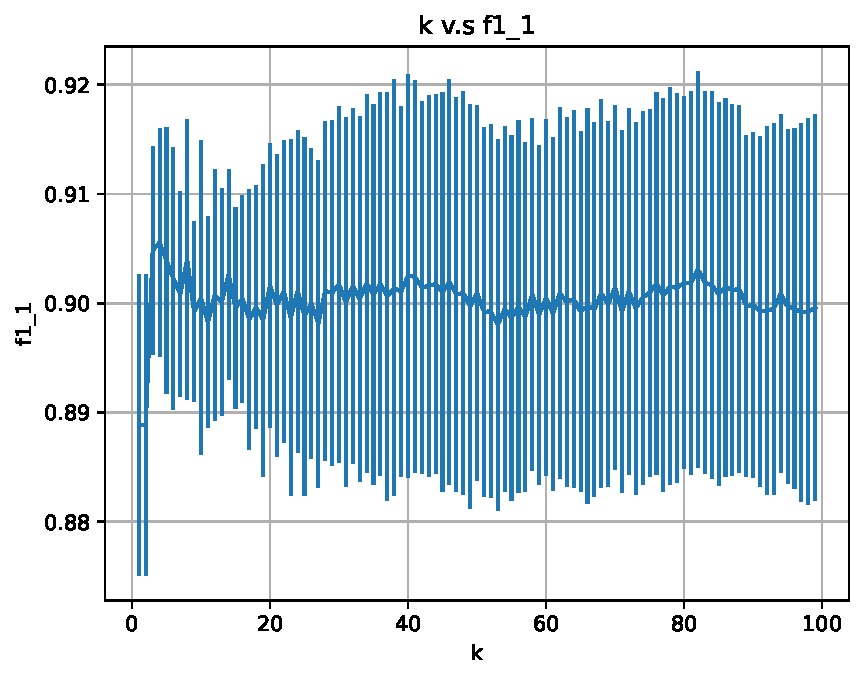
\includegraphics[width=0.30\textwidth]{figures/rice_knn_f1_1.pdf}
    \caption{Performance metrics graphed against k for KNN on the rice dataset.}
    \label{fig:rice_knn}
\end{figure}

\begin{figure}
    \centering
    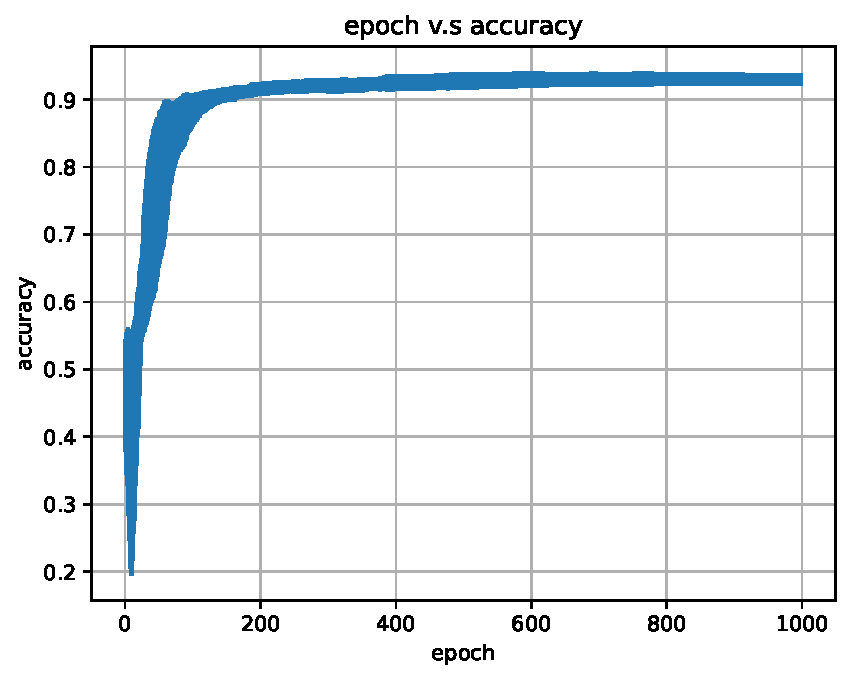
\includegraphics[width=0.30\textwidth]{figures/rice_nn_accuracy.pdf}
    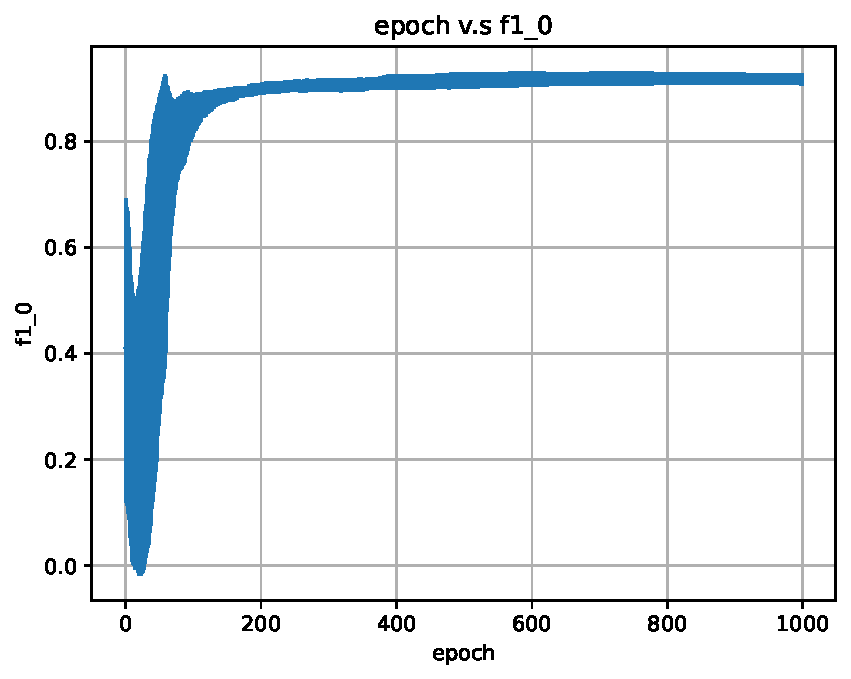
\includegraphics[width=0.30\textwidth]{figures/rice_nn_f1_0.pdf}
    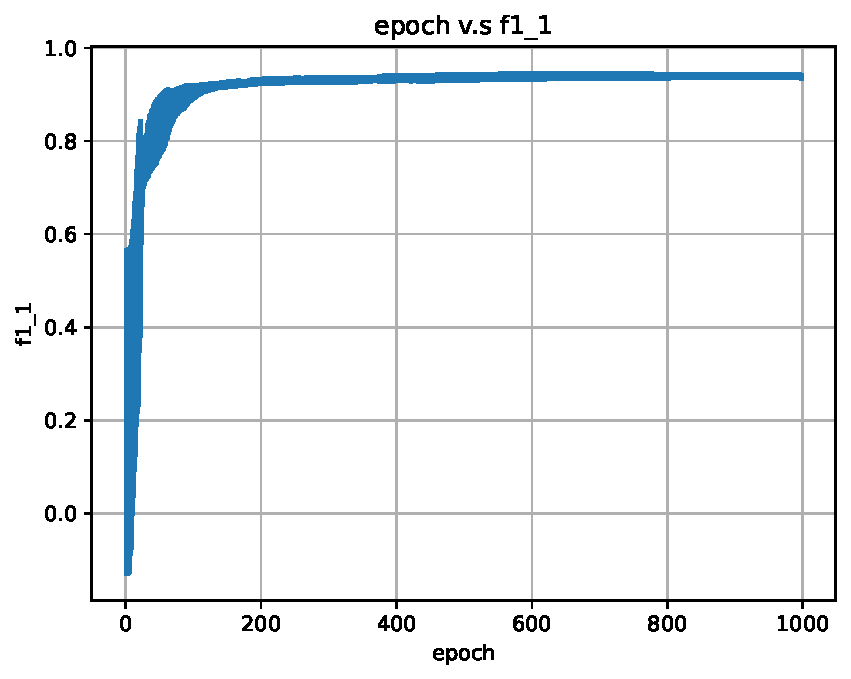
\includegraphics[width=0.30\textwidth]{figures/rice_nn_f1_1.pdf}
    \caption{Training graphs for a MLP trained on the rice dataset.}
    \label{fig:rice_nn}
\end{figure}

\begin{figure}
    \centering
    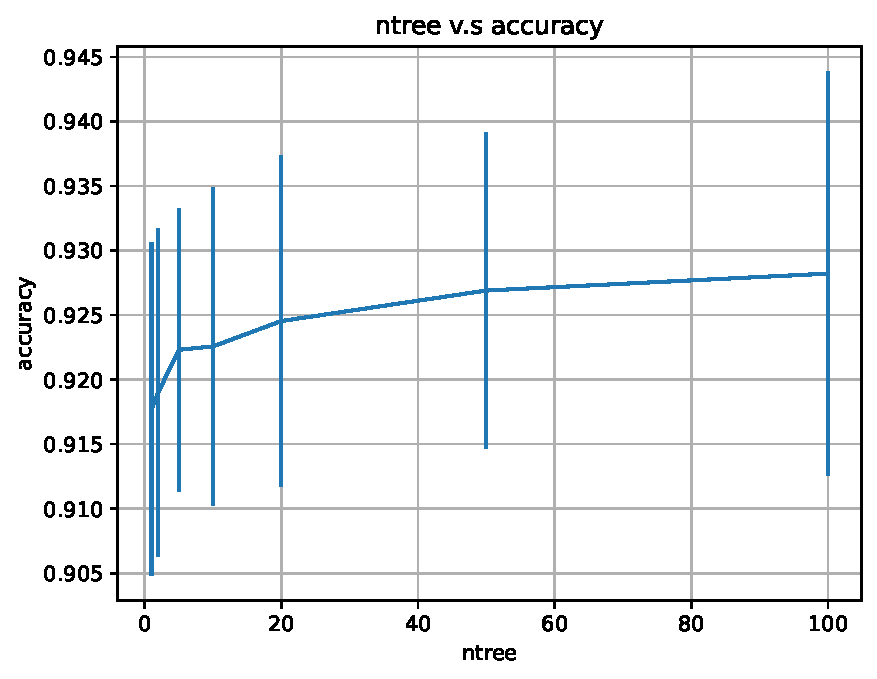
\includegraphics[width=0.30\textwidth]{figures/rice_random_forest_accuracy.pdf}
    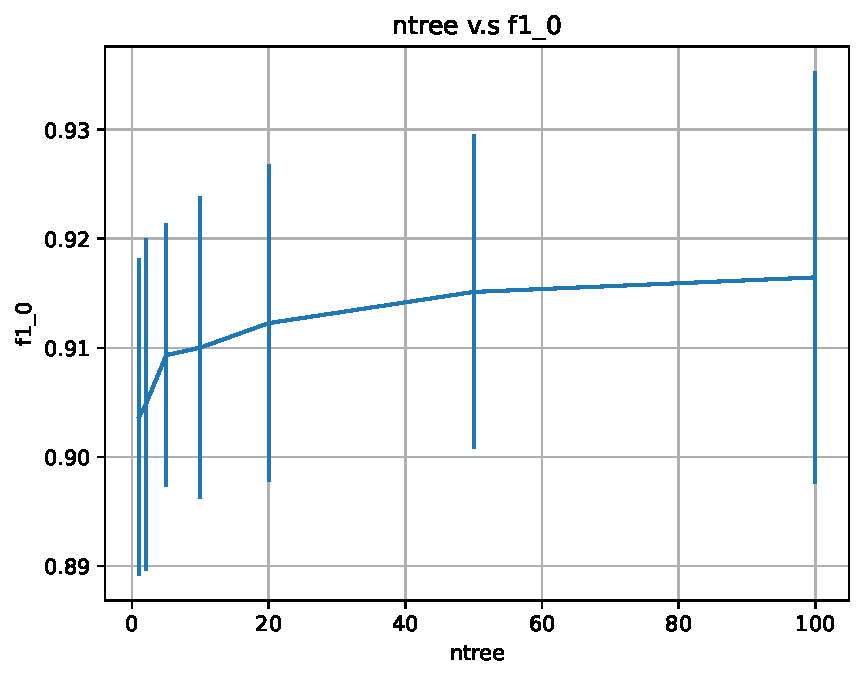
\includegraphics[width=0.30\textwidth]{figures/rice_random_forest_f1_0.pdf}
    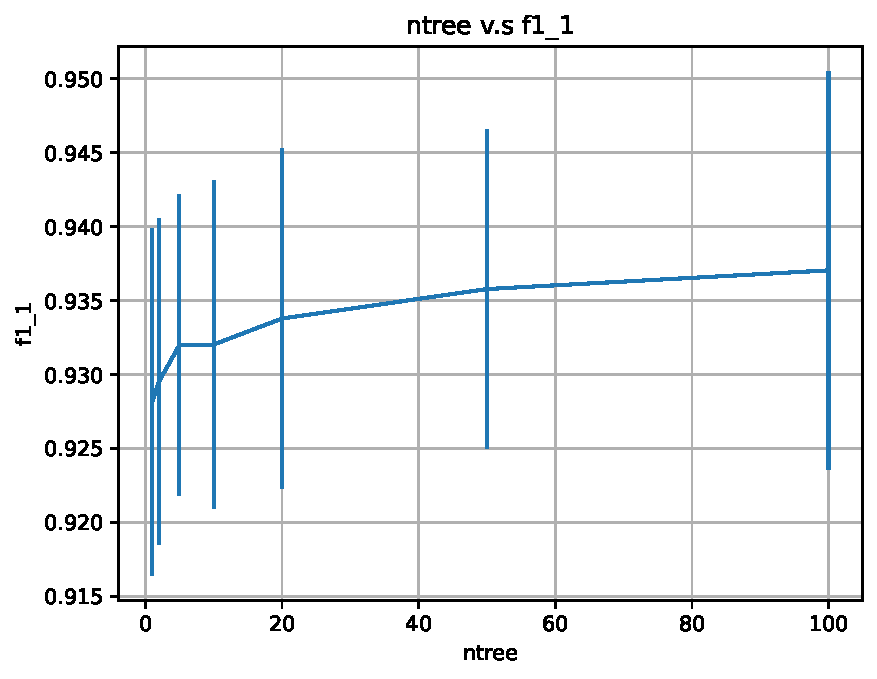
\includegraphics[width=0.30\textwidth]{figures/rice_random_forest_f1_1.pdf}
    \caption{Performance metrics graphed against ntree for random forests trained on the rice
             dataset}
    \label{fig:rice_random_forest}
\end{figure}
